%% \documentclass[crop,tikz]{standalone}
%% \begin{document}
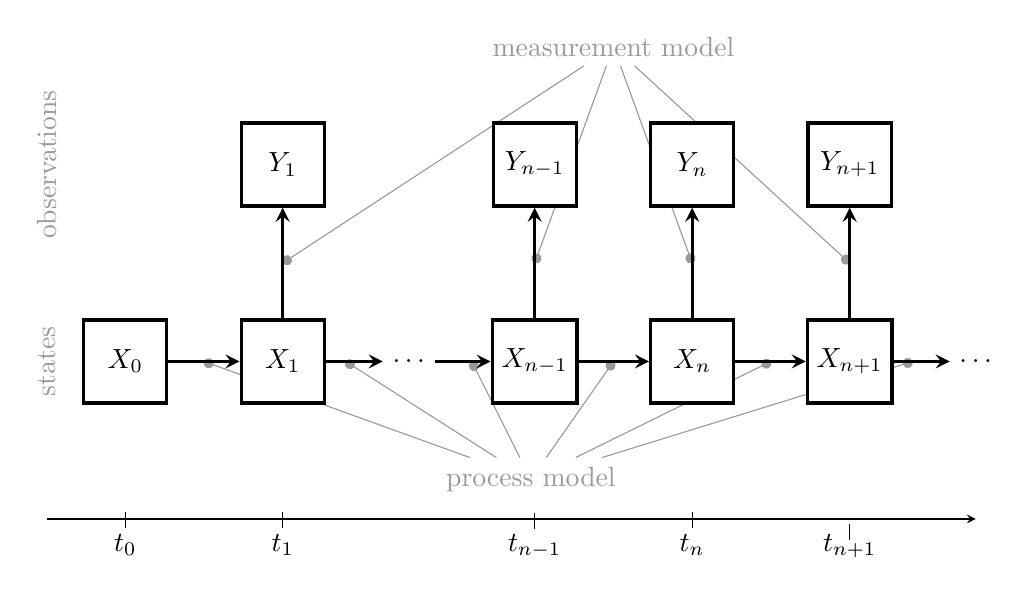
\begin{tikzpicture}[scale=1]
  \usetikzlibrary{arrows.meta,decorations,backgrounds,positioning,calc}

  \tikzstyle{box}=[draw=black, text=black, fill=white, very thick, minimum size=3em]
  \tikzstyle{label}=[font=\Large]
  \tikzstyle{coordinate}=[inner sep=0pt,outer sep=0pt]
  \tikzstyle{dep}=[draw=black, very thick, >=stealth]
  \tikzstyle{indicate}=[draw=black!40!white, >=Circle]
  \tikzstyle{lab}=[text=black!40!white]
  \tikzstyle{axis}=[draw=black, thin, >=stealth]
  \def\hsp{2}
  \def\vsp{2.5}

  \coordinate (origin) at (0,0);
  \node [box] (X0) at ($(origin)+(1,2)$) {$X_0$};
  \node [box] (X1) at ($(X0)+(\hsp,0)$) {$X_1$};
  \node [box] (Y1) at ($(X1)+(0,\vsp)$) {$Y_1$};
  \node (dots) at ($(X1)+(1.6,0)$) {$\dots$};
  \node [box] (Xnm1) at ($(dots)+(1.6,0)$) {$X_{n-1}$};
  \node [box] (Ynm1) at ($(Xnm1)+(0,\vsp)$) {$Y_{n-1}$};
  \node [box] (Xn) at ($(Xnm1)+(\hsp,0)$) {$X_{n}$};
  \node [box] (Yn) at ($(Xn)+(0,\vsp)$) {$Y_{n}$};
  \node [box] (Xnp1) at ($(Xn)+(\hsp,0)$) {$X_{n+1}$};
  \node [box] (Ynp1) at ($(Xnp1)+(0,\vsp)$) {$Y_{n+1}$};
  \node (dots2) at ($(Xnp1)+(1.6,0)$) {$\dots$};
  \draw [dep,->] (X0) -- (X1);
  \draw [dep,->] (X1) -- (dots);
  \draw [dep,->] (X1) -- (Y1);
  \draw [dep,->] (dots) -- (Xnm1);
  \draw [dep,->] (Xnm1) -- (Xn);
  \draw [dep,->] (Xnm1) -- (Ynm1);
  \draw [dep,->] (Xn) -- (Xnp1);
  \draw [dep,->] (Xn) -- (Yn);
  \draw [dep,->] (Xnp1) -- (dots2);
  \draw [dep,->] (Xnp1) -- (Ynp1);
  \node [lab,rotate=90] (lslab) at ($(X0)+(-1,0)$) {states};
  \node [lab,rotate=90] (obslab) at ($(lslab)+(0,\vsp)$) {observations};
  \draw [axis,->] (origin) -- (dots2 |- origin);
  \node [below=2pt of X0 |- origin] (t0) {$t_0$};
  \draw [axis] ($(t0)+(0,6pt)$) -- +(0,6pt);
  \node [below=2pt of X1 |- origin] (t1) {$t_1$};
  \draw [axis] ($(t1)+(0,6pt)$) -- +(0,6pt);
  \node [below=2pt of Xnm1 |- origin] (tnm1) {$t_{n-1}$};
  \draw [axis] ($(tnm1)+(0,6pt)$) -- +(0,6pt);
  \node [below=2pt of Xn |- origin] (tn) {$t_{n}$};
  \draw [axis] ($(tn)+(0,6pt)$) -- +(0,6pt);
  \node [below=2pt of Xnp1 |- origin] (tnp1) {$t_{n+1}$};
  \draw [axis] ($(tnp1)+(0,2pt)$) -- +(0,6pt);
  \begin{scope}[on background layer]
    \node [lab,right=10pt] (pmlab) at ($(dots)+(0,-1.5)$) {process model};
    \draw [indicate,->] (pmlab) -- ($(X0)!0.5!(X1)$);
    \draw [indicate,->] (pmlab) -- ($(X1)!0.5!(dots)$);
    \draw [indicate,->] (pmlab) -- ($(dots)!0.5!(Xnm1)$);
    \draw [indicate,->] (pmlab) -- ($(Xnm1)!0.5!(Xn)$);
    \draw [indicate,->] (pmlab) -- ($(Xn)!0.5!(Xnp1)$);
    \draw [indicate,->] (pmlab) -- ($(Xnp1)!0.5!(dots2)$);
    \node [lab] (mmlab) at ($(Ynm1)+(1,1.5)$) {measurement model};
    \draw [indicate,->] (mmlab) -- ($(X1)!0.5!(Y1)$);
    \draw [indicate,->] (mmlab) -- ($(Xnm1)!0.5!(Ynm1)$);
    \draw [indicate,->] (mmlab) -- ($(Xn)!0.5!(Yn)$);
    \draw [indicate,->] (mmlab) -- ($(Xnp1)!0.5!(Ynp1)$);
  \end{scope}
\end{tikzpicture}
%% \end{document}
